\section{Deterministic Solvers}
In this section we identify the four deterministic solvers on which uncertainty propagation will be applied.

\subsection{Polynomial Solver}
We include this test case because of the analytic solution, mean, and variance.  Since we treat a solver as a black box accepting inputs and returning outputs, evaluating a polynomial is a very simple test case.
The solver performs one of the two function evaluations, depending on the number of uncertain variables:
\begin{align}
f(x) &= 1+2x,\\
f(x,y) &=x\qty(1+y).
\end{align}
The analytic first and second moments of the functions $f(x)$ and $f(x,y)$ are shown in Table \ref{tab:polymoments}.
\begin{table}[H]
\centering
\begin{tabular}{c|c|c}
Function & $\expv{f}$ & $\expv{f^2}$ \\ \hline
$f(x)$ & $1+2\expv{x}$ & $1+4\expv{x}+4\expv{x^2}$ \\
$f(x,y)$ & $\expv{x}\qty(1+\expv{x})$ & $\expv{x^2}\qty(1+2\expv{y}+\expv{y^2})$
\end{tabular}
\caption{First and Second Moments of Polynomial Solvers}
\label{tab:polymoments}
\end{table}

\subsection{Source Solver}
Like polynomial solvers, this solver evaluates a simple expression; however, there are several potential uncertain terms.  Because the solution $U$ varies nonlinearly with some of the terms, a polynomial expansion of finite degree cannot exactly represent the solution.  This solver is the analytic solution to an isotropic monoenergetic neutron source spread homogeneously throughout a purely absorbing one-dimensional semi-infinite medium.  The governing PDE is
\begin{equation}
-D\ddrv{\phi}{x}+\Sigma_a\phi = S.
\end{equation}
The unknown is the scalar flux $\phi$.  $D$ is the diffusion coefficient, $\Sigma_a$ is the macroscopic absorbing cross section, and the forcing term $S$ is the homogenous source strength.  Boundary conditions include no-traction on the left and TODO on the right.  The solution at any particular point $x$ is given by
\begin{equation}
\phi=\frac{S}{\Sigma_a}\left(1-e^{-x/L}\right),
\end{equation}
\begin{equation}
L^2= \frac{D}{\Sigma_a}.
\end{equation}
We can summarize this solver as
\begin{equation}
\phi=\phi\qty(S,D,x,\Sigma_a),\hspace{10pt}\phi\in\mathbb{R}.
\end{equation}

\subsection{1D Diffusion Solver}
This problem is a simple version of a $k$-eigenvalue criticality problem using 1D, two-energy diffusion for neutron transport.  While this problem is 1D, we use a 2D mesh to solve it by imposing reflecting boundary conditions on the top and bottom, with vacuum (no-traction) boundaries on the right and left.  We also consider only one homogeneous material for the entire mesh.  The governing PDE for this equation is
\begin{equation}
-\drv{}{x}D_g\drv{\phi_g}{x}+(\Sigma_{g,a}+\Sigma_{g,s})\phi_g = \sum_{g'}\sigma_{s}^{g'\to g}\phi_{g'} + \frac{\chi_{g}}{k(\phi)}\sum_{g'}\nu_{g'}\sigma_{f,g'}\phi_{g'},\hspace{15pt} g\in[1,2],
\end{equation}
\begin{equation}
\Sigma_{g,a}=\Sigma_{g,c}+\Sigma_{g,f},
\end{equation}
The unknown is the two-vector angular flux $\phi=(\phi_1,\phi_2)$ and the quantity of interest is criticality eigenvalue $k(\phi)$.  Group index $g$ denotes the energy group; $D$ is the group diffusion cross section; $x$ is the location within the problem; $\Sigma_a,\Sigma_s,\Sigma_f,\Sigma_c$ are the macroscopic absorption, scattering, fission, and capture cross sections respectively; and $\chi$ is the fraction of neutrons born into an energy group.  In this case, we consider only downscattering, and fission neutrons are only born into the high energy group ($\Sigma_s^{2\to1}=\chi_2=0$).

The input parameters for this solver include all the material properties ($D_g,\Sigma_{g,c},\Sigma_{g,s},\Sigma_{g,f},\nu_g$), $g=1,2$.  The output parameter is $k$.  We can summarize this solver as 
\begin{equation}
k=k\qty(D_g,\Sigma_{g,c},\Sigma_{g'\to g,s},\Sigma_{g,f},\nu_g),\hspace{10pt}g\in(1,2),\hspace{10pt}k\in\mathbb{R}.
\end{equation}

\subsection{Quarter Core Solver}
The last solver acts on the PDEs most often used in approximating nuclear reactor behavior.  In particular, we consider a two-dimensional $k$-eigenvalue steady state problem with two energy groups.  The domain is square as
\begin{equation}
D=[0,200\text{ cm}]^2,
\end{equation}
and is shown in Fig. \ref{core}.  We assign the labels top, bottom, left, and right to corresponding locations in Fig. \ref{core}.
\begin{figure}[H]
\centering
   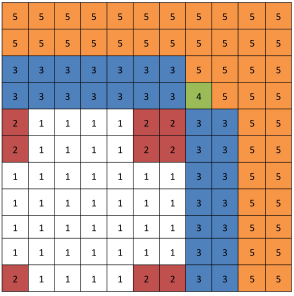
\includegraphics[width=0.3\textwidth]{../graphics/core}
   \caption{Problem Domain}
   \label{core}
\end{figure}

We consider all fission neutrons to be initialized with fast energies, and disregard up-scattering in energy.  Our coupled PDEs are
\begin{equation}
-\grad D_1^{(R)}\grad\phi_1(\bar x)+(\xs{1,a}{R}+\xs{1\to2,s}{R})\phi_1(\bar x) = \frac{1}{k(\phi)}\sum_{g'=1}^2\nu_{g'}^{(R)}\xs{g',f}{R}\phi_{g'}(\bar x),
\end{equation}
\begin{equation}
-\grad D_2^{(R)}\grad \phi_2(\bar x)+\xs{2,a}{R}\phi_2(\bar x) = \xs{1\to 2,s}{R}\phi_1(\bar x).
\end{equation}
We impose reflecting boundary conditions on the left and bottom, and vacuum (or no-traction) boundaries on the top and right, defined by
\begin{align}
\text{Vacuum: }&-D\eval{\pdv{\phi}{x_1}}_{x_1=0}=0,\\
&-D\eval{\pdv{\phi}{x_2}}_{x_2=0}=0,
\end{align}
\begin{align}
\text{Reflective: }&\eval{\pdv{\phi}{x_1}}_{x_1=0}=0,\\
&\eval{\pdv{\phi}{x_2}}_{x_2=0}=0.
\end{align}

The unknown is the two-vector $\phi=(\phi_1,\phi_2)^T$ and the quantity of interest $k$ is the criticality eigenvalue, given by
\begin{equation}
k(\phi)=\sum_{g=1}^2\iint\limits_D\nu\xs{f}{g}\phi(x_1,x_2)dxdy,
\end{equation}
Group index $g\in(1,2)$ denotes the energy group of the property; material index $R(\bar x)\in(1,2,3,4,5)$ is the material of the property; $D$ is the neutron diffusion cross section; $\phi(\bar x)$ is the scalar neutron flux measured in neutrons per area per time;  $\nu$ is the average number of neutrons produced per fission; $\xs{g'\to g,s}{R}$ is the macroscopic neutron interaction cross section for neutrons with initial energy in group $g'$ transitioning to energy group $g$ in material $R$; $\xs{g,f}{R}$ is the macroscopic neutron fission cross section for neutrons in energy group $g$ for material $R$; and $\xs{g,a}{R}$ is the total neutron absorption interaction cross section for group $g$ in material $R$, which is further given by the macroscopic capture and fission cross sections as
\begin{equation}
\xs{g,a}{R}\equiv\xs{g,c}{R}+\xs{g,f}{R},\hspace{10pt} g=1,2.
\end{equation}
We can summarize this solver as
\begin{equation}
k=k\qty(D_g^{(R)},\xs{g,c}{R},\xs{g'\to g,s}{R},\xs{g,f}{R},\nu_g^{(R)}),\hspace{10pt} g\in(1,2),R\in(1,2,3,4,5),\hspace{10pt}k\in\mathbb{R}.
\end{equation}
